\documentclass[tikz,border=2pt]{standalone}
\usepackage{libertinus}
\usepackage{tikz}

\begin{document}

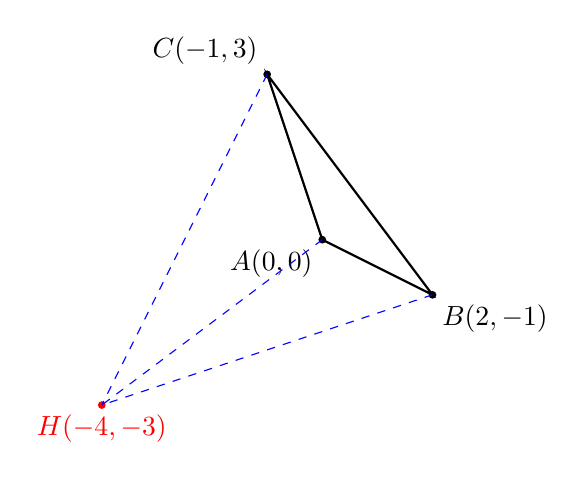
\begin{tikzpicture}[scale=0.7]

  % Points
  \coordinate (A) at (0,0);
  \coordinate (B) at (2,-1);
  \coordinate (C) at (-1,3);
  \coordinate (H) at (-4,-3);

  % Triangle
  \draw[thick] (A)--(B)--(C)--cycle;

  % Vertices
  \fill (A) circle (2pt) node[below left] {$A(0,0)$};
  \fill (B) circle (2pt) node[below right] {$B(2,-1)$};
  \fill (C) circle (2pt) node[above left] {$C(-1,3)$};

  % Orthocenter
  \fill[red] (H) circle (2pt) node[below] {$H(-4,-3)$};

  % Altitudes
  \draw[dashed,blue] (A)--(H);
  \draw[dashed,blue] (B)--(H);
  \draw[dashed,blue] (C)--(H);

\end{tikzpicture}

\end{document}
